\documentclass[border=10pt]{standalone}
\usepackage[svgnames]{xcolor}
\usepackage{amsmath}
\usepackage{pgfplots}
\pgfplotsset{compat=newest}
\usepackage[sfdefault]{FiraSans}
\usepackage{FiraMono}
\renewcommand*\familydefault{\sfdefault}
\begin{document}
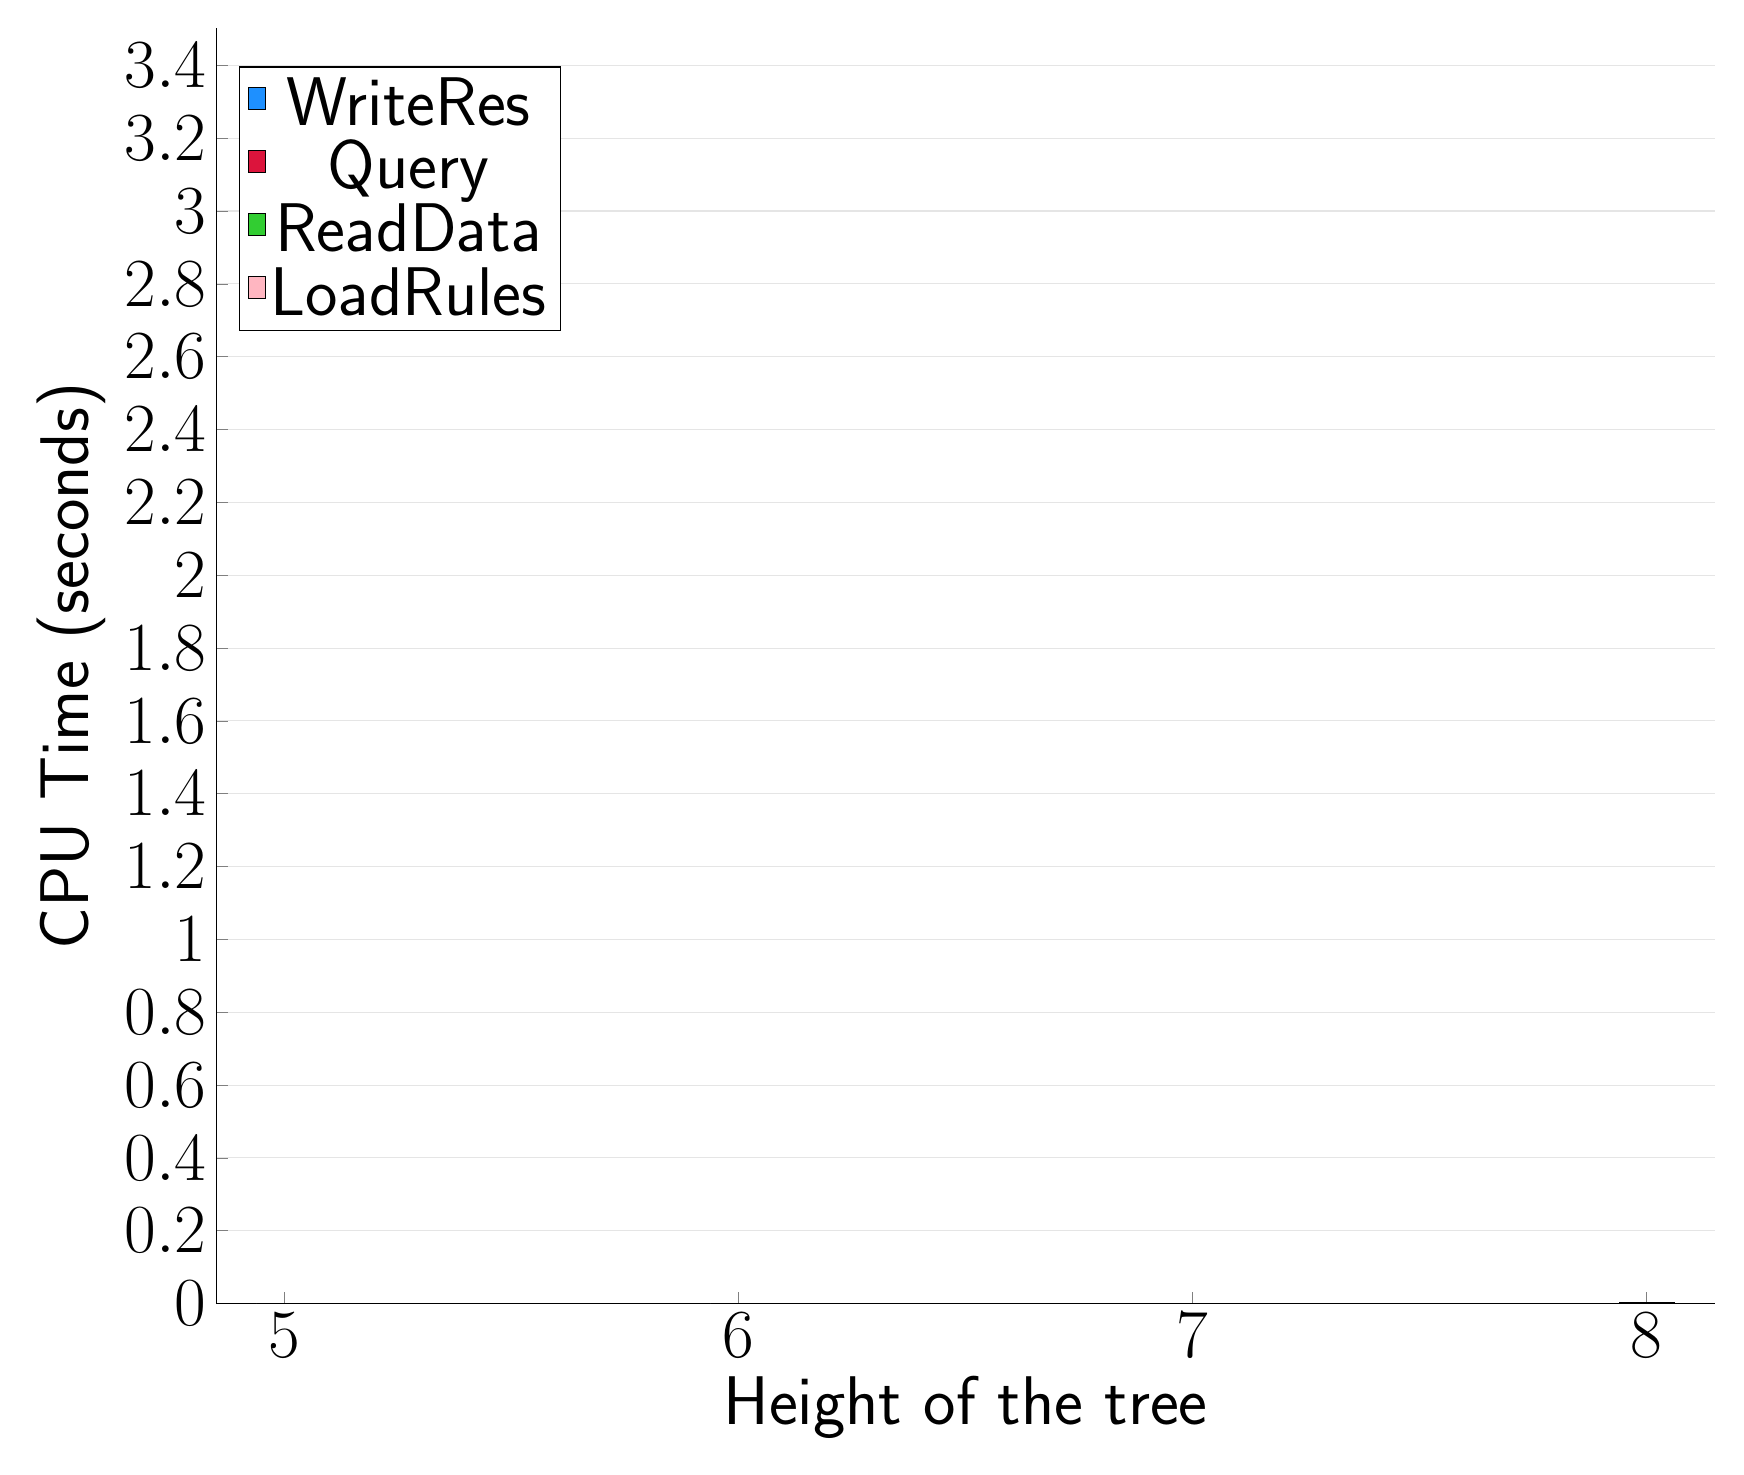
\begin{tikzpicture}
\begin{axis}[
   ybar stacked,
   width=1.7\textwidth,
   bar width=0.7cm,
   ymajorgrids, tick align=inside,
   major grid style={draw=gray!20},
   xtick=data,
   ymin=0, ymax=3.5020000000000002,
   axis x line*=bottom,
   axis y line*=left,
   enlarge x limits=0.05,
   legend style={
       at={(0.23, 0.97)},
       anchor=north east,
       legend columns=1,
       font=\Huge,
   },
   ylabel={CPU Time (seconds)},
   xlabel={Height of the tree},
   label style={font=\Huge},
   tick label style={font=\Huge},
]
\addlegendimage{fill=DodgerBlue, draw=black, line width=0.2pt}
\addlegendentry{WriteRes}
\addlegendimage{fill=Crimson, draw=black, line width=0.2pt}
\addlegendentry{Query}
\addlegendimage{fill=LimeGreen, draw=black, line width=0.2pt}
\addlegendentry{ReadData}
\addlegendimage{fill=LightPink, draw=black, line width=0.2pt}
\addlegendentry{LoadRules}
\addplot +[fill=LightPink, draw=black, line width=0.2pt] coordinates {
(5, 0.0006007000000000003)
(6, 0.0005972000000000003)
(7, 0.0006123000000000003)
(7, 0.0006026000000000006)
(7, 0.0006090000000000004)
(8, 0.0005976000000000003)
(8, 0.0006092999999999999)
(8, 0.0006185000000000001)
};
\addplot +[fill=LimeGreen, draw=black, line width=0.2pt] coordinates {
(5, 0.00016139999999999978)
(6, 0.00018269999999999978)
(7, 0.00023829999999999972)
(7, 0.0002412999999999998)
(7, 0.00024109999999999982)
(8, 0.0003510000000000001)
(8, 0.0003514000000000001)
(8, 0.00035729999999999974)
};
\addplot +[fill=Crimson, draw=black, line width=0.2pt] coordinates {
(5, 2.2000000000000155e-05)
(6, 3.6000000000000096e-05)
(7, 6.960000000000042e-05)
(7, 6.920000000000019e-05)
(7, 6.950000000000014e-05)
(8, 0.00014489999999999992)
(8, 0.0001466)
(8, 0.0001489000000000004)
};
\addplot +[fill=DodgerBlue, draw=black, line width=0.2pt] coordinates {
(5, 0.0001561000000000001)
(6, 0.00030479999999999944)
(7, 0.0006472999999999997)
(7, 0.0006433999999999997)
(7, 0.0006484)
(8, 0.001446)
(8, 0.001462)
(8, 0.0014440999999999996)
};
\end{axis}
\end{tikzpicture}

\end{document}
